\documentclass[11pt,a4paper]{article}
\XeTeXlinebreaklocale "zh"
\XeTeXlinebreakskip = 0pt plus 1pt minus 0.1pt
\usepackage[top=1in,bottom=1in,left=1.25in,right=1.25in]{geometry}
\usepackage{float}
\usepackage{fontspec}
\newfontfamily\zhfont[BoldFont=STHeiti]{STFangsong}
\newfontfamily\zhpunctfont{STFangsong}
\setmainfont{Times New Roman}
\usepackage{indentfirst}
\usepackage{zhspacing}
\zhspacing

\usepackage[colorlinks=true]{hyperref}

% 代码展示
\usepackage{color}
\definecolor{bg}{rgb}{0.152941, 0.156863, 0.133333}
\usepackage{minted}
\usemintedstyle{monokai}
\setmonofont{DejaVuSansMono}

\usepackage{fancyvrb}  % 调整 Verbatim 中字体

% 调整 quotation 字体
\let\quotationOLD\quotation
\def\quotation{\quotationOLD\footnotesize}

\usepackage{pdfpages}  % 附上 pdf 版综合结果

\renewcommand{\figurename}{图 }  % 图片标题

\begin{document}

\title{实验四\ \ 串口收发器设计}
\author{无36$\quad$李思涵$\quad$2013011187}
\maketitle

\section{实验目的}
\begin{itemize}
  \item 了解和掌握 UART 的工作原理。
\end{itemize}

\section{设计方案}
\subsection{原理说明}
本次实验中,主要任务在于实现串口数据的接受和发送。下面是实验指导书中的原理说明。

\subsubsection{串口基本原理}
\begin{quotation}
  “UART(Universal Asynchronous Receiver/Transmitter)是一种通用串行数据总线,用于异步通信。该总线双向通信,可以实现全双工传输和接收。在嵌入式设计中,UART用来与PC进行通信,包括与监控调试器和其它器件。与UART相关的一个概念是RS232-C标准,该标准由美国电子工业协会EIA(Electronic Industry Association)制定的一种串行物理接口标准,其规定了若干标准的数据速率,并且采用较高电平来保证20米以内的有线传输。

  UART是计算机与嵌入式系统中串行通信端口的关键部分,速率有规定的9600等波特率。在实际应用中,通用串口的电气特性兼容RS232规范信号,即逻辑“1”信号相对于地为 -3 到 -15 伏,而逻辑“0”相对于地为3到15伏。因此,当一个微控制器的UART与外界电路相连时,需要采用一个符合RS232标准的驱动器来将控制器管脚的CMOS电平或TTL电平转换为 RS232 标准电平。TTL电平是3.3V的,而RS232是负逻辑电平,如果没有类似MAX232的驱动芯片进行电平转换,这么高的电压很可能会把芯片烧坏。

  发送一个完整的字节信息,首先是一个作为起始位的逻辑“0”位,接着是8个数据位,然后是1个、1+1/2个或2个停止位逻辑“1”位,数据线空闲时呈现为高或“1”状态。在字符的8位数据部分,先发送数据的最低位(LSB),最后发送最高位(MSB)。每位持续的时间是固定的,由发送器本地时钟控制,每秒发送的数据位个数,即为“波特率”。

  起始位和停止位起着很重要的作用。显然,他们标志每个字符的开始和结束,但更重要的是他们使接收器能把局部时钟与每个新开始接收的字符再同步。异步通信没有可参照的时钟信号,发送器随时都可能发送数据,需要从任何边沿的出现时刻开始正确地采样紧接着的 10~11位(包括开始位、数据位和停止位)。接收器的时钟与发送器的时钟不是同一个,因此,接收器采样点的间隔跟由发送器时钟所确定的位间隔时间不同,接收器设计不好可能会导致采样错误。”
\end{quotation}

\subsubsection{Nexys3 开发板相关电路介绍}
\begin{quotation}
  “FT232是FTDI公司的串口转USB芯片,FPGA(Spartan6)通过其与PC机上的串口通用程序通信。在PC机一侧通过串口调试助手选择对应的USB COM端口,设置波特率为9600,1位停止位,无硬件数据流控,无奇偶校验”
\end{quotation}

\subsubsection{实验设计原理}
\begin{quotation}
  “串口收发器包括发送器和接收器两个模块。首先,通过串口接收器模块从外部接收数据,并将接收到的数据送给控制器模块,同时控制器模块根据接收的串口数据产生发送数据,并通过串口发送器模块将数据发送到外部。

  串口接收器(UART Receiver)模块负责从串口中接收串行数据流,并根据UART通讯协议提取接收到的数据并发送给控制器。每当串口接收器收到一个完整的数据,在 RX\_STATUS 上输出一个高电平指示脉冲,并同时在 RX\_DATA 上输出接收到的有效数据, RX\_DATA 上的接收数据一直有效到下一个 RX\_STATUS 脉冲位置。

  由于从线路上接收到的串行数据帧与接收模块的时钟是异步的,所以接收器功能实现中的关键是接收器时钟与每个接收字符的同步。一个有效的方法是接收器采用高速率时钟对串行数据进行采样,通常采样频率是位时钟频率的整数倍。理论上倍数越高接收数据各位的分
  辨率越高,实际中,一般最大选择16倍。波特率发生器(Baud Rate Generator)模块负责根据System clock时钟产生所需的16倍(或者其他倍数)波特率的接收时钟。

  接收器应该尽可能地在靠近位周期的中心处对每位采样。如果接收器能很好地预测起始位的开始,那么可在起始位的下降沿到来之后,等待半个位周期再采样数据位。此后,接收器每等待一个位周期采样一个数据位,直至收到最后一位为止。倘若接收时钟的频率足够接近发送时钟,使得最后位能在离该位的精确中心位置半个周期内对他采样,以上方案就能正确地工作。这意味着接收时钟相对于发送时钟在10~11个时钟周期内,其增加和减少应小于半个位的时间间隔。因此,要求收发双方2个时钟的误差容限在 5\% 以内。

  串口发送器(UART Sender)从控制器接收待发送数据,然后根据UART通讯协议串行发送出去。当控制器检测到 TX\_STATUS 上出现高电平时,意味着此时串口发送器处于空闲状态可以接收一个新的发送数据,控制器在 TX\_DATA 上输出待发送的数据,并同时在 TX\_EN 上输出一个高电平脉冲,指示串口发送器启动一个新的数据发送。”
\end{quotation}

从上面的原理可以看出,实现串口收发器的主要难点在于串口数据的接受。这是因为,数据可能会在任何时间到达串口接收器,并且发送端和接收端的时钟很可能不同步。因为,为了能够较好地接受串口数据,应该对接收到的信号进行采样。并且,采样最好能发生在一个每个数据位的中心,这样能够在两个方向都有比较大的时钟误差容限。

结合上实验原理,我最后选择了这样的采样方案:用 FSM 实现采样器,其有三个状态,分别为
\begin{description}
  \item[STANDING\_BY] 等待起始位到来;
  \item[PADDING] 接收到起始位,填充半个数据周期的空白,从而移动到数据位的中心;
  \item[SAMPLING] 采样,每隔一个数据周期输出一个脉冲采样信号。
\end{description}

而接收器则在采样信号的上升沿对数据进行采样,将数据保存并计数。当累计接收到 8 个数据位之后,将接收到的数据传递给控制模块,并用  RX\_STATUS 信号指示接收完成了一个字节的数据。

控制模块则在接受到新数据之后对其进行处理,并转发给发送模块;发送模块则在接受到使能信号之后开始以 9600 的波特率发送串口信号,并在发送期间保持 TX\_STATUS 为0。

需要注意的是,只要能保证发送模块能在 10 个数据周期之内完成一字节信号的发送(1 起始位 + 8 数据位 + 1 终止位),控制模块便不需要检测发送模块是否空闲。事实上,如果没有达到这个要求,串口收发器便不能对连续发送的串口信号进行持续的接受和发送。所以,保证发送模块的高效性也是十分关键的。

\subsection{框图}
图~\ref{fig:串口收发器功能实现框图} 表示了串口收发器的结构。可以看到,整个收发器主要由三个部分组成:接收模块,控制模块和发送模块。

\begin{figure}[htb]
  \centering
    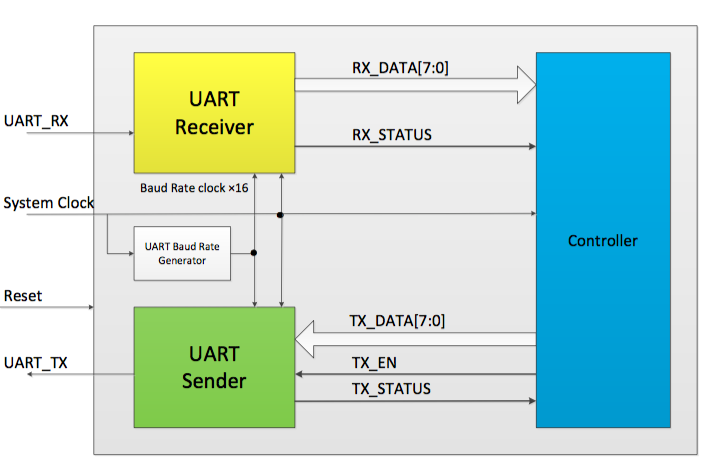
\includegraphics[width=\textwidth]{structure}
  \caption{串口收发器功能实现框图}
  \label{fig:串口收发器功能实现框图}
\end{figure}


\section{关键代码}

\subsection{采样器状态机部分的实现}

\begin{minted}[bgcolor=bg, linenos=true, fontsize=\footnotesize]{verilog}
reg [1:0] state, next_state;
localparam STANDING_BY = 2'd0,
           PADDING = 2'd1,
           SAMPLING = 2'd2;

// Assume SAMPLE_RATIO <= 16
reg [3:0] count = 0, next_count,
          bit_count = 0, next_bit_count;
wire next_sample_sig;

// Calculate next values.
always @(*) begin
    case (state)
    STANDING_BY: begin
        next_state = (din ? STANDING_BY : PADDING);
        next_count = 4'b0;
        next_bit_count = 4'b0;
    end

    PADDING: begin  // Wait PADDING_TIME clk.
        if (count < PADDING_TIME - 1) begin
            next_state = PADDING;
            next_count = count + 4'b1;
        end else begin
            next_state = SAMPLING;
            next_count = 4'b0;
        end
        next_bit_count = 4'b0;
    end

    SAMPLING: begin  // Cycle = SAMPLE_RATIO.
        next_state = (bit_count == 4'd9 ? STANDING_BY : SAMPLING);

        if (count < SAMPLE_RATIO - 1) begin
            next_count = count + 4'b1;
            next_bit_count = bit_count;
        end else begin
            next_count = 4'b0;
            next_bit_count = bit_count + 4'b1;
        end
    end

    default: begin
        next_state = 0;
        next_count = 0;
        next_bit_count = 0;
    end
    endcase
end

assign next_sample_sig = (state == SAMPLING &&
                          count == SAMPLE_RATIO - 4'd2 &&
                          bit_count < 4'd8);

// Update values.
always @(posedge sample_clk) begin
    state <= next_state;
    count <= next_count;
    bit_count <= next_bit_count;
    sample_sig <= next_sample_sig;
end
\end{minted}

可以看到,这里确实使用了状态机来实现采样器。需要注意的是,这里一共有四个状态变量:state, count, bit\_count 和 sample\_sig,其保存的分别是当前阶段,采样时钟计数,数据位计数和采样信号。

这里要注意,sample\_sig 被实现成了一个状态而不是一个组合电路。这是因为 sample\_sig 将会被当做时钟使用。若用组合电路来实现,其值很可能发生抖动,从而导致上层接收模块被错误地触发。将其作为状态保证了它的值只会被同步更新,从而避免了抖动。


\subsection{发送器的实现}

\begin{minted}[bgcolor=bg, linenos=true, fontsize=\footnotesize]{verilog}
// 1 padding, 1 start-bit, 8 data-bits, 1 end-bit.
localparam COUNTER_MAX = 4'd11;

reg [8:0] shift_reg;
assign dout = shift_reg[0];

reg [3:0] counter = 0;
wire rst_n = ~tx_en;

always @(posedge send_clk or negedge rst_n) begin
    if(~rst_n) begin
        counter <= 0;
    end else begin
        if (counter == 4'b0)
            shift_reg <= {tx_data, 1'b0};  // Load data.
        else
            shift_reg <= {1'b1, shift_reg[8:1]};  // Shift.

        if (counter < COUNTER_MAX)
            counter <= counter + 4'b1;
        else
            counter <= counter;
    end
end

always @(posedge clk) begin
    tx_status <= (counter < COUNTER_MAX ? 1'b0 : 1'b1);
end
\end{minted}

发送器具体采用的是移位寄存器的实现方式。需要注意的是,由于接收器是在接受完了最后一位数据后立刻更新了状态,所以计数器是被异步清零的。为了保证发出的串口信号能有一位的起始位,这里加入了一位填充位。

乍看起来,这样做会导致发送一个数据需要 11 个数据周期,不符合连续收发的要求。但实际上,在十个数据周期以后,数据已经被完全发送了,还未发送的只有终止位。若信号足够紧凑,则下一个使能信号回来下一个数据周期中到来,而只有 counter 会被清零,移位寄存器的值在这个周期内并不会变,所以终止位仍能正常发出。

换一句话说,计数器值为 0 和 10 时对应的输出相同,故可以被提前终止,从而达到最小 10 个数据周期的要求。

\section{文件清单}

\begin{Verbatim}[fontsize=\scriptsize]
exp4
└── serial_transceiver
    ├── Makefile
    ├── hex_led.v
    ├── receiver.v
    ├── receiver_tb.v
    ├── sampler.v
    ├── sampler_tb.v
    ├── sender.v
    ├── sender_tb.v
    ├── serial_transceiver.bit
    ├── serial_transceiver.ucf
    ├── serial_transceiver.v
    ├── serial_transceiver_tb.v
    └── sim

common
├── bcd7.v
└── watchmaker.v
\end{Verbatim}

其中 Makefile 用来构建仿真程序,sim 文件为 Icarus Verilog 生成的仿真程序。

其中,receiver\_tb.v, sampler\_tb.v 和 sender\_tb.v 是子模块的测试套件,是验证小模块正确性写的,采用的参数与最终测试略有不同,故没有附上仿真结果。


\section{仿真结果及分析}
使用的仿真工具为:Icarus Verilog 0.9.7 \& Modelsim 10.3c

仿真结果如下:

\subsection{Icarus Verilog 仿真结果}
\VerbatimInput[fontsize=\scriptsize, numbers=left]
{../../exp4/serial_transceiver/result.txt}

\subsection{Modelsim 仿真结果}
\begin{figure}[htb]
  \centering
    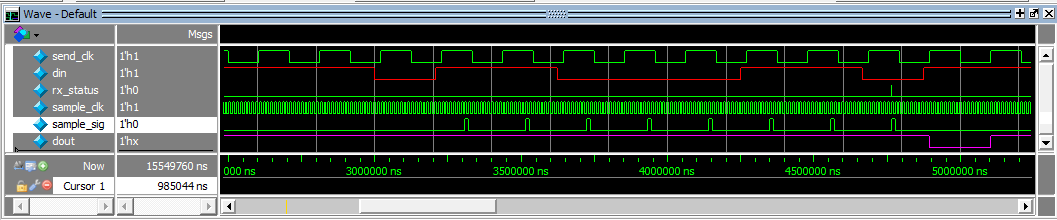
\includegraphics[width=\textwidth]{exp4_receive_wave}
  \caption{接收波形}
  \label{fig:接收波形}
\end{figure}

从图~\ref{fig:接收波形} 中可以看出,采样器确实能够很好地预测数据到来的时间,能够准确地在数据位的中间进行发生采样脉冲。

\begin{figure}[htb]
  \centering
    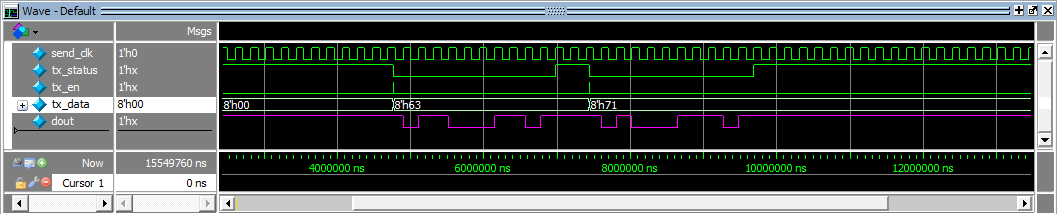
\includegraphics[width=\textwidth]{exp4_send_wave}
  \caption{发送波形}
  \label{fig:发送波形}
\end{figure}

从图~\ref{fig:发送波形} 中可以看到,在 tx\_en 脉冲以及新的 tx\_data 到来后,tx\_status 迅速变成了 0,并开始在 dout 上发送串行信号。

\begin{figure}[htb]
  \centering
    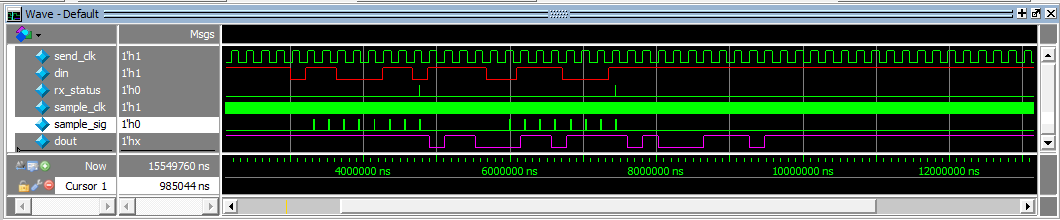
\includegraphics[width=\textwidth]{exp4_wave}
  \caption{总波形}
  \label{fig:总波形}
\end{figure}

从图~\ref{fig:总波形} 中可以看出,我们的串口收发器在仿真中确实实现了要求的功能,并能够对较密集的输入流进行处理(没有测试最密集的情况,即两字节之间没有间隔)。


\section{综合情况}
见附页。

\section{硬件调试情况}
由于早就听说这个实验比较难,我早早地开始了实验。

由于考虑得比较清楚,整个系统的设计并没有走太多的弯路。设计出来的代码也经过了两个仿真器的检验,应该是万无一失了…

但是!!!

但是烧到板子上之后,他不工作啊啊啊啊啊啊…

花了一整个周六 debug,用实验平台上的 LED 灯来调试,甚至还找了学长…

但是它就是接受不到任何数据啊啊啊啊啊啊啊啊啊啊啊啊啊啊啊啊啊啊啊啊啊啊啊啊啊

当时要死的心都有了…

最后在网上查的时候,发现别人说的管脚和我的不太一样= =

“我可是再三核对过管脚的哇”,疑惑的我再次打开了指导书,找到了配图。

……

原来 UART 接受数据的意思是接受板子发送的数据?!?!

……

于是改了端口就能用了……

后来又因为采样模块采样时钟抖动的问题修改了一下设计,然后又改了改发送器使其能连续发送数据。

最后因为实在不甘心,便做了一个比较炫酷的显示:

数码管用 16 进制显示接收到的字节 \& 发送出的字节

8 个 LED 管则有 4 档功能,用两个开关切换,分别是:

\begin{itemize}
  \item 输入字节二进制表示
  \item 输出字节二进制表示
  \item 发送器的当前状态 (tx\_status)
  \item 收发器的当前负载(像温度计一样!对数表示当前负载!十分炫酷!)
\end{itemize}

心好累…但总算是做完了…

Cheers \textasciitilde

\includepdf[pages={-}]{serial_transceiver.pdf}

\end{document}

